\begin{defn}[Predicates]
    A \emph{predicate}\index{predicate} is a statement containing a finite number of variables. The predicate becomes true or false based on the value of the variables.
\end{defn}
\begin{exposition}[Sample Predicates]
Find values for the variables which make the predicates true or false.
\begin{sides}
    \begin{itemize}
    \setlength{\itemsep}{18pt}
        \item \(P(x): x\in\bbZ \wedge x>5\)
        \item \(Q(x): x\in\bbR \wedge x>5\)
        \item \(G(a,b):  a>b\)
        \item \(\forall a,b\in\bbZ: G(a,b) \rightarrow G(a^3,b^3)\)
        \item \(S(n,m): n^2>m\)
    \end{itemize}
\tcblower
    \begin{itemize}
    \setlength{\itemsep}{18pt}
        \item \(\exists n\in\bbZ: S(n,25)\)
        \item \(\forall n\in\bbZ: S(n,0)\)
        \item \(\exists n\in\bbZ: \sim S(n,0)\)
        \item \(\forall a,b\in R: G(a,b)\leftrightarrow S(a,b)\)
        \item \(\forall n\in\bbN\ \exists a,b,c\in\bbZ: a^n+b^n=c^n\)
    \end{itemize}
\end{sides}    
\end{exposition}

\begin{practiceprob}[Shapes, Colors, and Zombies, Oh My!!]
Use figure \ref{fig:Tarski} on page \pageref{fig:Tarski} to identify when these predicates are true or false.
\begin{sides}
    \begin{itemize}
    \setlength{\itemsep}{18pt}
        \item \(C(x):\) \(x\) is a consonant
        \item \(V(x):\) \(x\) is a vowel
        \item \(Z(x):\) \(x\) is a zombie
        \item \(S(x):\) \(x\) is a stick figure
        \item \(N(x):\) \(x\) is a brain
        \item \(R(x):\) \(x\) is \textcolor{red!60!black}{\bfseries\em red}
    \end{itemize}
    \tcblower
    \begin{itemize}
    \setlength{\itemsep}{18pt}
        \item \(B(x):\) \(x\) is \textcolor{blue!50!black}{\em\bfseries blue}
        \item \(G(x):\) \(x\) is \textcolor{green!60!black}{\bfseries\em green}
        \item \(P(x):\) \(x\) is a pentagon (5-sides)
        \item \(H(x):\) \(x\) is a heptagon (7-sides)
        \item \(W(x,y):\) \(x\) is in the same row as \(y\)
        \item \(L(x,y):\) \(x\) is in the same column as \(y\)
    \end{itemize}
\end{sides}
\end{practiceprob}

\clearpage

\begin{figure}[H]
    \centering
    % \inputtikz{tarski_world}
    \includegraphics[scale=0.06,alt={Ten by ten grid with various shapes letters and figures},width=0.9\linewidth]{images/created/tarski_world.png}
    \caption{Tarski's World}
    \label{fig:Tarski}
\end{figure}

\clearpage

\begin{exposition}[Truth Sets]

Given a predicate, the \emph{truth set}\index{truth set} for that predicate is the collection of all elements where it is true.  For example for \(V(x): x\ \text{is a vowel}\), the truth set is 
    \[T_V=\left\{a,e,i,o,u,y\right\}\] and for \(P(x): x\ \text{is a pentagon}\) the truth set is \[T_P=\left\{t,a,u,h,k,o,p\right\}.\] 
Figure \ref{fig:VP_Venn} shows how these two sets are related, in particular we can see that 
    \[V(x)\wedge P(x)\ \text{and}\ V(x)\wedge \sim P(x)\ \text{and}\ \sim V(x)\wedge P(x)\]
are all true if we pick the right value of \(x\).

\begin{figure}[H]
    \centering
    % \inputtikz{truth_set_venn}
    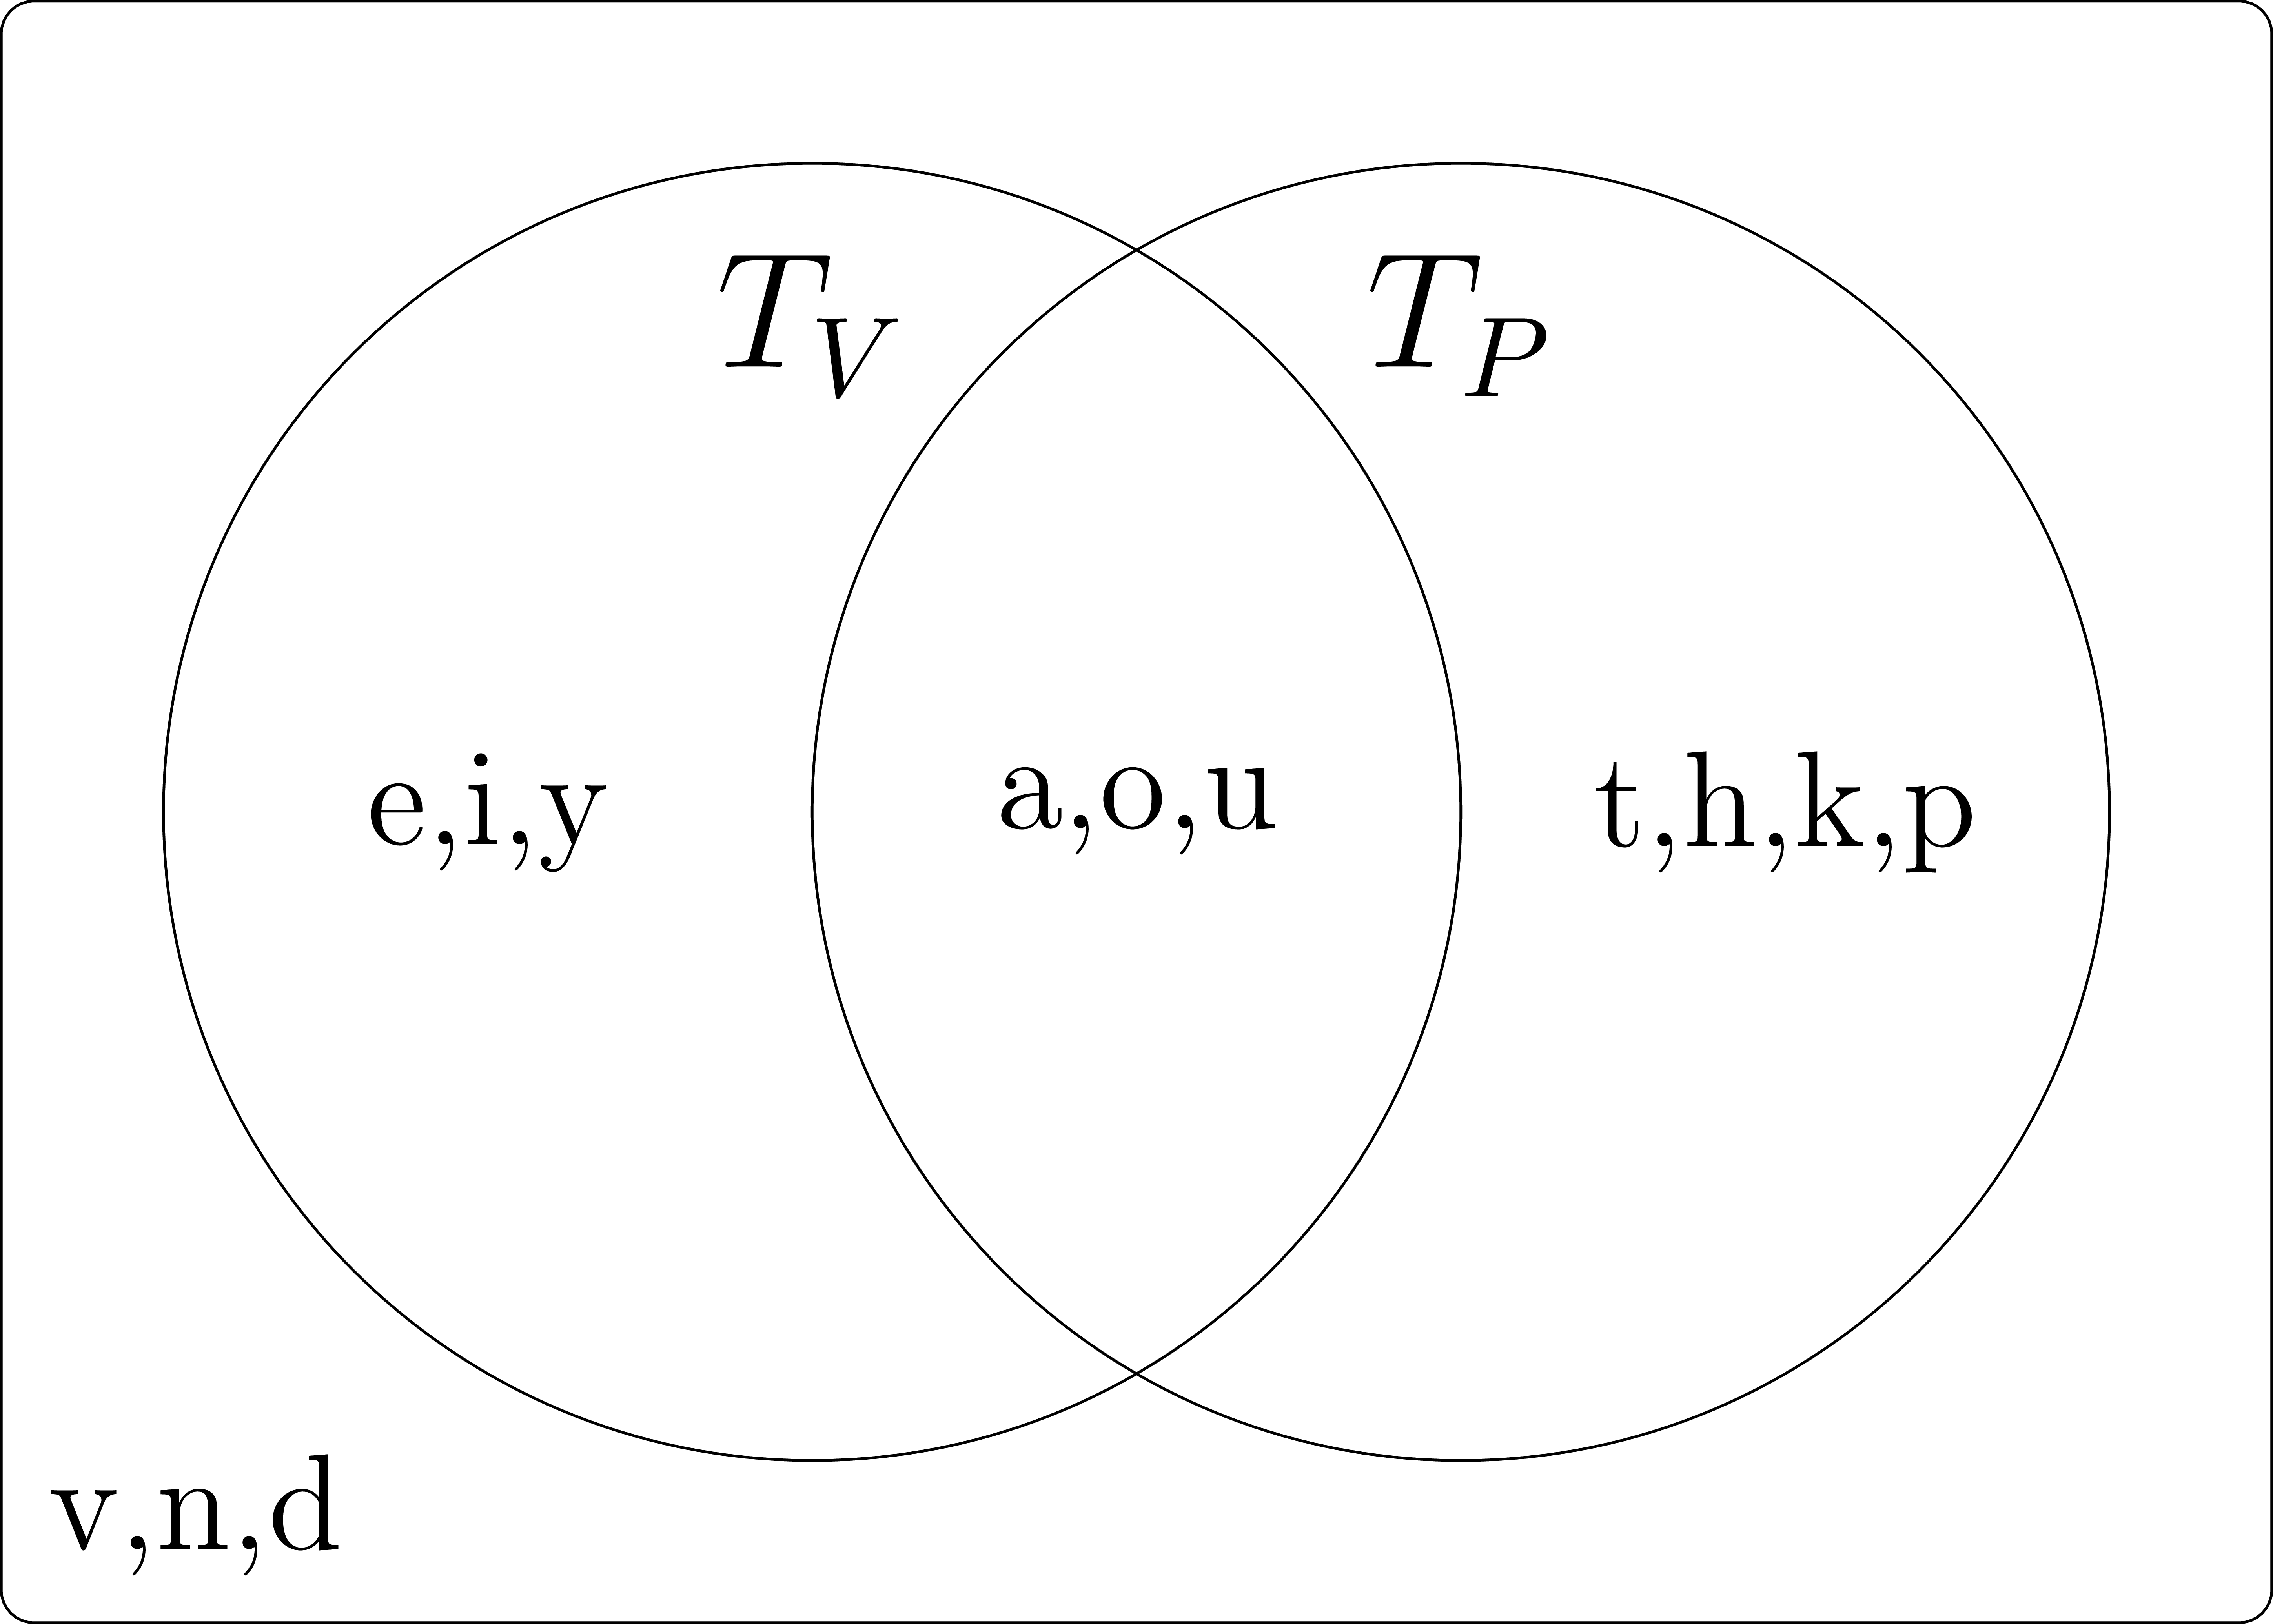
\includegraphics[scale=0.06,alt={Venn diagram of two truth sets},width=0.75\linewidth]{images/created/truth_set_venn.png}
    \caption{Venn Diagram of \(T_V\) and \(T_P\)}
    \label{fig:VP_Venn}
\end{figure}





\noindent
The predicates like \[W(x,y):\, x\ \text{is in the same row as}\ y\]
would have the truth set
\[T_W=\left\{(e,h),(h,e),(u,p),(p,u),(i,k),(k,i),(a,d),(d,a),(t,o),(o,t)\right\}.\]
\end{exposition}

\clearpage

\begin{practiceprob}[Truth Zombies]
Using figure \ref{fig:Tarski}, fill in the \emph{truth set} for each of the predicates.
\begin{enumerate}
    \item The truth set for \(G(x)\) is \[T_G=\left\{\phantom{\rule{0.8\textwidth}{20pt}}\right\}\]
    \item The truth set for \(H(x)\) is \[T_H=\left\{\phantom{\rule{0.8\textwidth}{20pt}}\right\}\]
    \item Fill in the Venn Diagram in figure \ref{fig:GH_Venn} for each of the previous truth sets.
    \item Where would the set \(T_Z\) fit in figure \ref{fig:GH_Venn}?  What does that tell us about the statement \[\forall x: Z(x)\rightarrow G(x)?\]
    \item The truth set for \(L(x,y)\) is \[ T_L=\left\{\phantom{\rule{0.8\textwidth}{20pt}}\right\}\]
\end{enumerate}
\begin{figure}[H]
    \centering
    % \inputtikz{empty_truth_venn}
    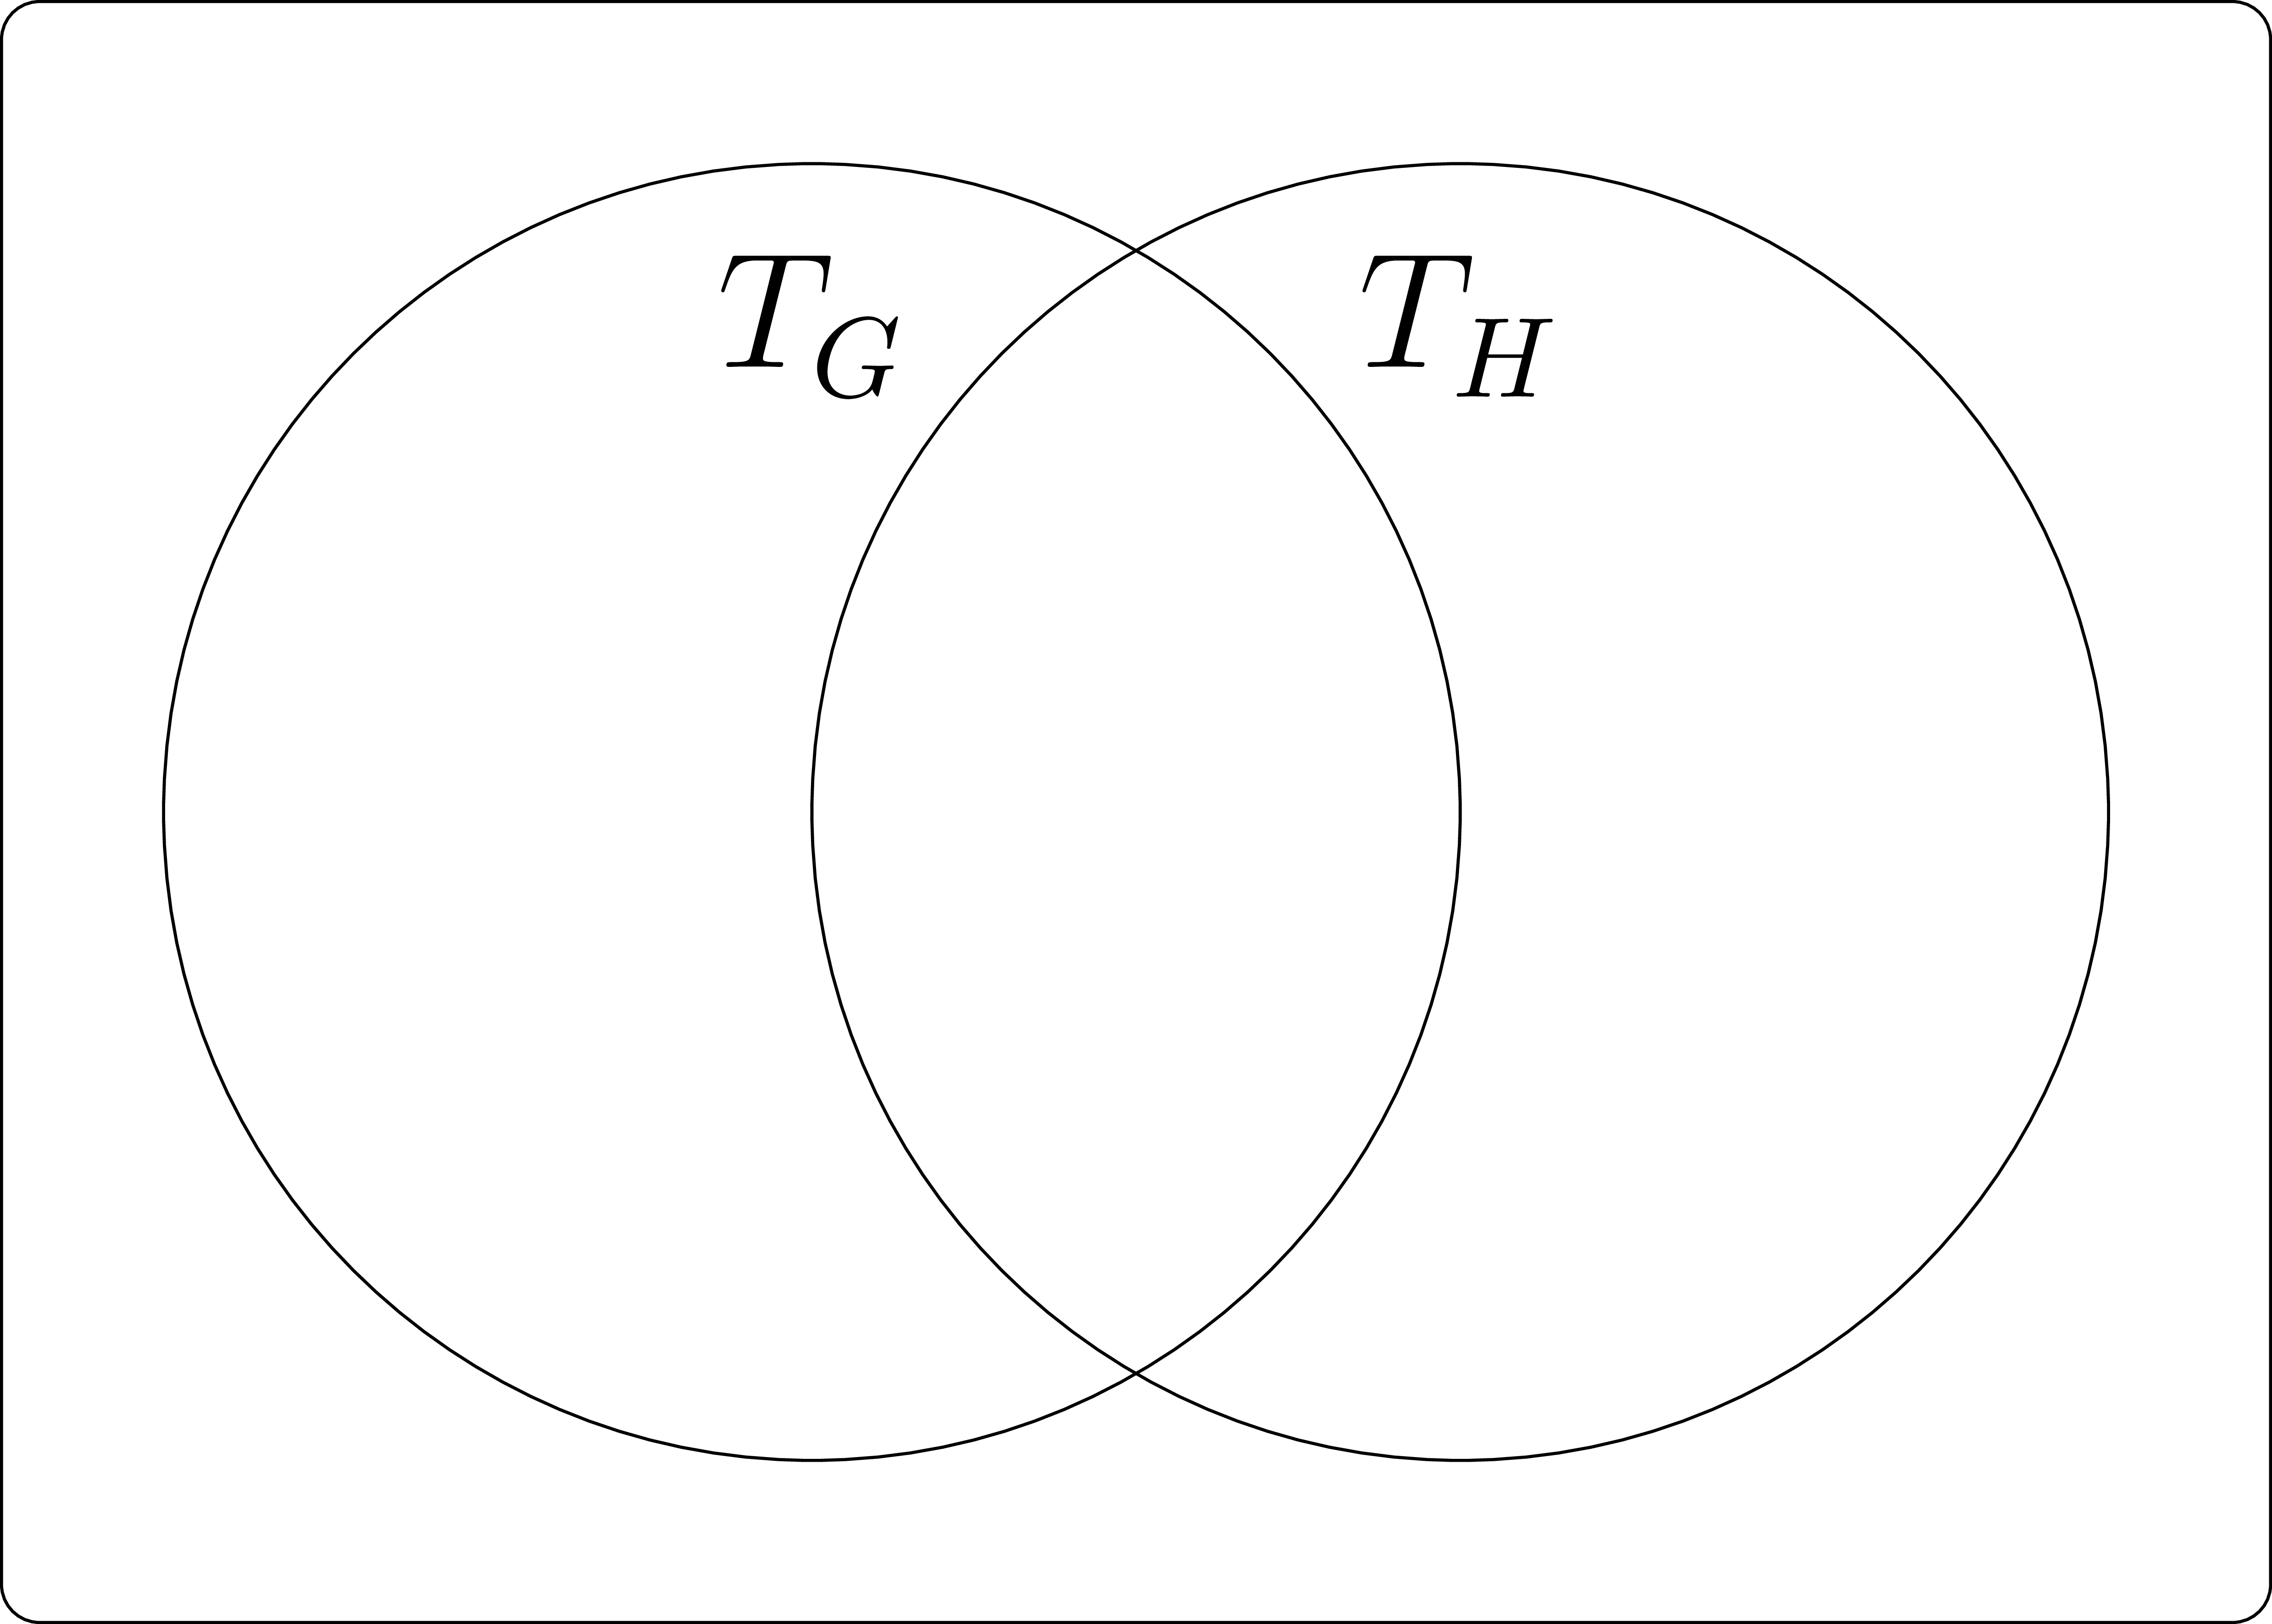
\includegraphics[scale=0.06,alt={Blank venn diagram for two truth sets},width=0.75\linewidth]{images/created/empty_truth_venn.png}
    \caption{Venn Diagram of \(T_G\) and \(T_H\)}
    \label{fig:GH_Venn}
\end{figure}
\end{practiceprob}

\clearpage

\begin{exposition}[Quantified Predicates]
% Examples
Recall \(\exists\) is the \emph{existential quantifier}\index{existential quantifier} and \(\forall\) the \emph{universal quantifier}\index{universal quantifier}.  Now, if we write 
    \[\exists x: V(x)\wedge P(x)\]
we can read that as 
\begin{center}
    \textit{``there exists a vowel which is also a pentagon''}
\end{center} 
or in plainer English 
\begin{center}
    \textit{``some vowels are pentagons.''}
\end{center} 
Is the previous statement true or false? How can we see it in the Venn Diagram in figure \ref{fig:VP_Venn}?\vspace{3\baselineskip}

\noindent
And, if we write 
    \[\forall x: V(x)\vee P(x)\]
we read it as 
\begin{center}
    \textit{``all the shapes are vowels or pentagons.''}
\end{center} Is this true or false? How can we see it in the Venn diagram in figure \ref{fig:VP_Venn}?\vspace{3\baselineskip}

\noindent
In addition to using them one at a time we can combine them like this 
    \[\forall x\,  \exists y: C(x)\rightarrow L(x,y)\] 
which we read as 
\begin{center}
    \textit{``every consonant shares a column with some letter,''}
\end{center} or like this \[\exists y\, \forall x: C(x)\rightarrow L(x,y)\] which we read as 
\begin{center}
    \textit{``some letter shares a column with every consonant.''}
\end{center} Which of the previous two statements is true and which is false?  How do we know?\vspace{3\baselineskip}
\end{exposition}

\clearpage

\begin{practiceprob}[Tarski's Zombies]
% Exercises
Referring to figure \ref{fig:Tarski}, which of the following predicates are true and which are false?  Try to write each in plain English and negate the false predicates.
\begin{enumerate}
\setlength{\itemsep}{40pt}
    \item \(\displaystyle\forall x: H(x)\rightarrow C(x)\)
    \item \(\displaystyle\exists x: V(x)\wedge R(x)\)
    \item \(\displaystyle\forall x\, \exists y: C(x)\rightarrow V(y)\wedge L(x,y)\)
    \item \(\displaystyle\forall x\, \forall y: C(x)\wedge V(y)\rightarrow L(x,y)\vee W(x,y)\)
    \item \(\displaystyle\forall x\in T_Z, \exists y\in T_N: W(x,y)\)
    \item \(\displaystyle\exists y\in T_N, \forall x\in T_Z: W(x,y)\)\vspace{35pt}
\end{enumerate}
Finally, look at figure \ref{fig:Tarski} and construct three quantified statements of your own using the given predicates.  Make two of them true and one a lie.  Make at least one of them doubly quantified.
\begin{itemize}
\setlength{\itemsep}{40pt}
    \item Truth:
    \item Truth:
    \item Lie:\vspace{35pt}
\end{itemize}
\end{practiceprob}

